\documentclass{ximera}
 
\input{../preamble.tex}
 
\title{Introduction to SPC}
 
\begin{document}
\begin{abstract}
\end{abstract}
 
\maketitle

\section*{Introduction to Statistical Process Control (SPC)}

\emph{Statistical Process Control} (SPC) is a methodology used in quality management to monitor and control a process to ensure it operates within specified limits and produces {\bf consistent} and {\bf predictable} results. It is widely used in various industries, including manufacturing, healthcare, and services, to maintain quality standards and improve process performance.

By collecting and analyzing data over time, SPC helps identify patterns, trends, and variations in the process that may affect product quality. It focuses on understanding the inherent variability in a process rather than relying solely on inspection and testing of finished products.

The main objectives of SPC are:
\begin{enumerate}

\item {\bf Monitoring:} SPC involves regularly collecting data from the process to monitor its performance. This data can include measurements of key process parameters or quality characteristics of the output.

\item {\bf Control:} SPC uses statistical methods to determine whether a process is in control or out of control. In-control means that the process is operating within acceptable limits, while out-of-control indicates that the process is experiencing unusual variation.

\item {\bf Variation Reduction:} SPC helps identify the sources of process variation and guides efforts to reduce or eliminate them. By understanding the causes of variation, organizations can make targeted improvements to enhance process stability and consistency.
\end{enumerate}

\begin{center}
        \begin{tikzpicture}
\node[inner sep=0pt, anchor=base] (p1) at (0,0)
  {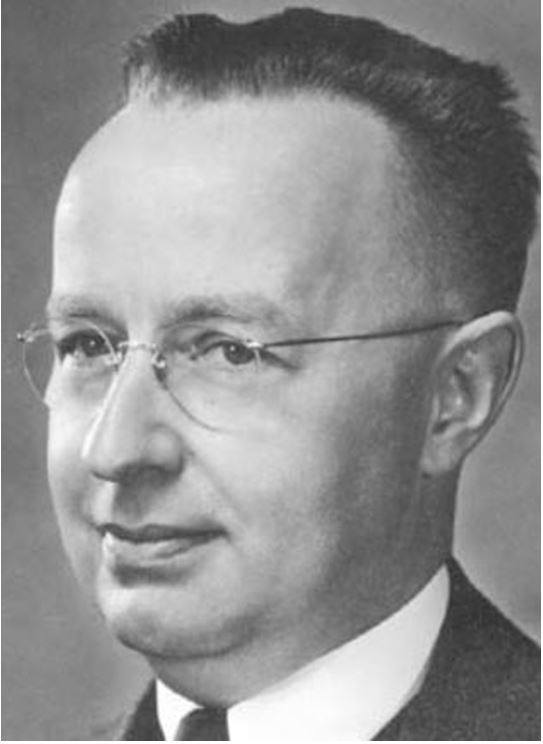
\includegraphics[height=70mm]{WAShewhart.jpg}};
  \node[] at (0,-0.5) (p2) {Walter A. Shewhart, 1891-1967};
         \end{tikzpicture}
      \end{center}

The concept of Statistical Process Control was developed by Dr. Walter A. Shewhart in the early 1920s. Dr. Shewhart was an American physicist, engineer, and statistician who worked at the Western Electric Company's Hawthorne Works in Chicago, Illinois, which was part of the Bell System. He is widely regarded as the pioneer of modern statistical quality control and is credited with the foundational principles and techniques of SPC.

Dr. Shewhart's work on SPC was primarily focused on addressing variation in manufacturing processes and improving product quality. He introduced the concept of \emph{control charts}, also referred to as \emph{quality control charts} (QCC), as a tool for monitoring and controlling variation in processes. Control charts are graphical representations of process data over time. They help visualize process performance, detect trends, and identify when the process goes out of control.

Dr. Shewhart's contributions to SPC laid the groundwork for subsequent developments in quality management and statistical techniques, and his ideas continue to be influential in the field to this day.

  The most commonly used control chart is the X-bar and R chart, which tracks the average and range of a variable.

 
\end{document}